\subsection{Maximum likelihood estimation in Gaussian graphical models}

A graphical model is a probabilistic model associating relations between random variables to a graph. The random variables of the model are represented by nodes in the graph and conditional independence relations are represented by missing edges between the corresponding nodes of the graph.

Consider a random vector $X$ distributed according to the \textit{multivariate Gaussian distribution} $N_p(0, \Omega^{-1})$, where the \textit{precision matrix} $\Omega \in \S^p_{\succ 0}$ is the inverse of the covariance matrix $\Sigma$. Thus, the density of $X$ is
\begin{equation} \label{eq-density-gaussian}
    f(x; \Omega) = (2\pi)^{-p/2} |\Omega|^{1/2} \expfc{-\frac{1}{2} \trB{xx^\top \Omega} }.
\end{equation}
Clearly, the multivariate Gaussian distribution is an exponential family with canonical parameter $\Omega$ and sufficient statistic $\frac{1}{2}xx^\top$. We start by stating a result about multivariate Normal distributions that can be found in \cite[Proposition C.5]{lauritzen1996}. 

\begin{lemma} \label{lem-gaussian-cond}
    Let $X \sim N_p(\mu, \Sigma)$ and $A, B \subset [p]$ be disjoint. Then, the conditional distribution of $X_A$ given $X_B = x_B$ is $N_{|A|}(\mu_{A|B}, \Sigma_{A|B})$ where
    \begin{align*}
        \mu_{A|B} = \mu_A + \Sigma_{A,B}\Sigma^{-1}_{B,B}(x_B - \mu_B) && \t{and} && \Sigma_{A|B} = \Sigma_{A,A} - \Sigma_{A,B}\Sigma^{-1}_{B,B}\Sigma_{B,A}.
    \end{align*} 
    One recognizes that the conditional covariance matrix $\Sigma_{A|B}$ is the Schur complement of $\Sigma_B$ in $\Sigma$.
\end{lemma}

We parametrize the multivariate Normal distribution in terms of the precision matrix because of its special role in the context of graphical models. Indeed, the conditional independence relations of the entries a random vector $X \sim N_p(0, \Omega)$ are characterized by the sparsity patterns of the precision matrix $\Omega$. This is shown in the following lemma from \cite[Proposition 5.2]{lauritzen1996}.
\
\begin{lemma}
    Let $X \sim N_p(\mu, \Sigma)$ and let $i, j \in [p]$ with $i \neq j$. Then
    \begin{equation} \label{eq-lemma-markov}
        \Omega_{ij} = 0 \iff X_i \independent X_j | X_{[p] \setminus \eset{i,j}}.
    \end{equation}
\end{lemma}
\begin{proof}
    By Lemma \ref{lem-gaussian-cond}, we have that the bivariate vector $X_{\eset{i,j}}$ is Gaussian with covariance matrix $\Sigma_{\eset{i,j}|[p]\setminus\eset{i,j}}$ equal to the Schur complement of $\Sigma_{[p] \setminus \eset{i,j}}$. The statement in (\ref{eq-lemma-markov}) is thus equivalent to 
    \begin{equation*}
        \Omega_{ij} = 0 \iff \Sigma_{\eset{i,j}|[p]\setminus\eset{i,j}}\ \t{is diagonal}.
    \end{equation*}
    Using the Schur complement inverse property, we have that
    \begin{equation*}
        \Sigma_{\eset{i,j}|[p]\setminus\eset{i,j}} 
        = \left[\Omega_{\eset{i,j}}\right]^{-1} 
        = \begin{pmatrix}
            \Omega_{ii} & \Omega_{ij}\\
            \Omega_{ji} & \Omega_{jj}
            \end{pmatrix}^{-1}
        = \frac{1}{|\Omega_{\eset{i,j}}|} \begin{pmatrix}
            \Omega_{jj} & -\Omega_{ij}\\
            -\Omega_{ji} & \Omega_{ii} 
            \end{pmatrix}^{-1}.
    \end{equation*}
    Hence, $\Sigma_{\eset{i,j}|[p]\setminus\eset{i,j}}$ is diagonal if and only if $\Omega_{ij} = 0$, completing the proof of the lemma.
\end{proof}

Consider a graph $\G = ([p], E)$. We say that $X$ satisfies the \textit{Gaussian graphical model} with graph $\G$ if $X \sim N_p(0, \Omega)$ and
\begin{equation} \label{eq-ggm}
    \Omega_{i j} = 0 \t{ for all } \eset{i,j} \notin E^*.
\end{equation}
Property (\ref{eq-ggm}) corresponds to the pairwise Markov property in graphical model theory \cite{lauritzen1996}. Note that the independence relations of the entries of $X$, the connectivity of the nodes in $\G$ and the sparsity pattern of $\Omega$ are all the same concept viewed from a different angle, which each on its own will help in studying them.

We now study properties of the maximum likelihood estimator in a Gaussian graphical model, largely the presentation of Uhler \cite[Section 9]{maathuis2018handbook}.

Consider a sample $X = (X_1, \ldots, X_n)$ from a Gaussian distribution. The log-likelihood function for a precision matrix $\Omega \in \S^p_{\succ 0}$ obtained from (\ref{eq-density-gaussian}) is
\begin{equation*}
    \ell(\Omega; X) = \frac{n}{2} \log |\Omega| - \frac{1}{2}\tr[XX^\top\Omega].
\end{equation*}
Rewriting the log-likelihood in terms of the sufficient statistic $S = n^{-1}XX^\top$, we get that
\begin{equation} \label{eq-likelihood}
    \ell(\Omega; S) = \frac{n}{2}\log |\Omega| - \frac{n}{2}\tr[S\Omega].
\end{equation}
In the \textit{saturated model} where no constraints are put on the entries of $\Omega$, the maximum likelihood estimator is defined when $S \in S^p_{\succ 0}$ and is equal to
\begin{equation*}
    \hat\Omega = S^{-1}.
\end{equation*}
Note that, if we are interested in estimating the maximum likelihood estimator $\hat\Omega$ of a Gaussian graphical model with graph $\G = ([p], E)$, the solution $\hat\Omega$ must lie in the subset $\S_{\succ 0}(\G)$ of $\S^p_{\succ 0}$ in which the conditional independence relations encoded in $\G$ are satisfied. We are left with the following optimization problem
\begin{align} \label{eq-primal}
    \begin{split}
        &\underset{\Omega \in \S^p_{\succ 0}}{\t{maximize}}\ \  \log |\Omega| - \tr[S\Omega]\\
        &\t{subject to}\ \ \Omega \in \S(\G).
    \end{split}
\end{align}
Since the Gaussian graphical model condition is a linear constraint, the set $\S(\G)$ is a convex cone. Showing that the objective function in (\ref{eq-primal}) is concave would imply that maximum likelihood estimation in Gaussian graphical models is a convex optimization problem. This would allow us to bring new insights to the maximum likelihood problem by studying its dual formulation. The following lemma from \cite[Proposition 9.2.1]{maathuis2018handbook} states that the objective function is indeed concave.
\begin{lemma}
    The function $f : \S^p_{\succ 0} \rightarrow \R, X \mapsto \log |X| - \trB{SX}$ is concave.
\end{lemma}
\begin{proof}
    Remark that the sum of a concave function and a linear function is concave, and $\trB{SX}$ is linear in $X$. Thus, it is sufficient to show that the logarithm of the determinant of a matrix is concave. To show this, we consider the line $\eset{ U + tV : t \in \R }$ for $U, V \in \S^p_{\succ 0}$. We show that $X \mapsto \log |X|$ is concave on $\S^p_{\succ 0}$ by proving that $g(t) = \log |U + tV|$ is concave as follows. Since $U \in \S^p_{\succ 0}$, both $U^{1/2}$ and $U^{-1/2}$ exist and we have 
    \begin{align*}
        g(t)
        &= \log |U + tV| \\
        &= \log |U^{1/2}(1_p + tU^{-1/2}VU^{-1/2}|\\
        &= \log |U| + \log |1_p + tU^{-1/2}VU^{-1/2}|.
    \end{align*}
    Let $\lambda_i$ be the eigenvalues of $U^{-1/2}VU^{-1/2}$ and note that the eigenvalues of $1_p + tU^{-1/2}VU^{-1/2}$ are $1 + t\lambda_i$. Therefore
    \begin{equation*}
        g(t) = \log |U| + \sum_{i=1}^p \log (1 + t\lambda_i).
    \end{equation*}
    Now, since each $\log (1 + t\lambda_i)$ is concave in $t$, we have that $g$ is concave, which completes the proof of the lemma.
\end{proof}

We can now study the dual problem to (\ref{eq-primal}). The Lagrangian of the likelihood maximization problem in Gaussian graphical models is given by
\begin{align*}
    \mathcal{L}(\Omega, \nu)
    &= \log |\Omega| - \tr[S\Omega] - 2 \sum_{\eset{i, j} \notin E} \nu_{ij}\Omega_{ij}\\
    &= \log |\Omega| - \sum_{i=1}^p S_{ii}\Omega_{ii} - 2 \sum_{\eset{i,j} \in E} S_{ij}\Omega_{ij} - 2 \sum_{\eset{i, j} \notin E} \nu_{ij}\Omega_{ij}
\end{align*}
The Lagrange dual $H$ of (\ref{eq-primal}) is given by $H(\nu) = \mathcal{L}(\Omega^\nu, \nu)$ where $\Omega^\nu$ is the maximizer of $\mathcal{L}(\Omega, \nu)$. Let $\Omega^\nu$ be the maximizer of $\mathcal{L}(\Omega, \nu)$ with respect to $\Omega$. Then, finding the roots $\Omega^\nu_{ij}$ of $\frac{\d}{\d\Omega_{ij}} \c{L}(\Omega, \nu)$ shows that the inverse $\Sigma^\nu$ of $\Omega^\nu$ satisfies the following
\begin{equation*}
    \Sigma^\nu_{ij} = \begin{cases}
        S_{ij}\ \t{ if } i = j \t{ or } \eset{i, j} \in E,\\
        \nu_{ij}\ \t{otherwise}.
    \end{cases}
\end{equation*}
Note that $\Sigma^\nu$ is the matrix formed by replacing entries in $S$ corresponding to missing edges with entries of the dual variables $\nu_{ij}$. Replacing $\Omega^\nu$ in the expression for the Lagrange dual function $H$, we obtain that
\begin{align*}
    H(\nu) 
    = \c{L}(\Omega^\nu, \nu)
    &= \log |\Omega^\nu| - \tr[S\Omega^\nu] - 2 \sum_{\eset{i, j} \notin E} \nu_{ij}\Omega^\nu_{ij}\\
    &= \log |\Omega^\nu| - \tr[\Sigma^\nu\Omega^\nu] + 2 \sum_{\eset{i, j} \notin E} \Sigma^\nu_{ij}\Omega^\nu_{ij} - 2 \sum_{\eset{i, j} \notin E} \nu_{ij}\Omega^\nu_{ij}\\
    &= \log |\Omega^\nu| - p = -\log |\Sigma^\nu| - p.
\end{align*}
Hence, the dual to (\ref{eq-primal}) is
\begin{align} \label{eq-dual}
    \begin{split}
        &\underset{\Sigma \in \S^p_{\succ 0}}{\t{minimize}}\ \  -\log |\Sigma| - p\\
        &\t{subject to}\ \ \Sigma_{ij} = S_{ij}\ \t{ for all } \eset{i, j} \in E^*.
    \end{split}
\end{align}
To prove that problems (\ref{eq-primal}) and (\ref{eq-dual}) are equivalent, we must show that strong duality holds for this convex optimization problem. By \textit{Slater's constraint quantification} \cite[Section 5.3.2]{boyd2004convex}, it is enough to show that there exists an $\Omega^* \in \S^p_{\succ 0}$ that is strictly feasable for the primal problem. Since the identity matrix is positive definite and is an element of $\S(\G)$ for any $\G$, strong duality holds for any graph $\G$. Thus, we can freely study both formulations of the optimization problem. Furthermore, Problems (\ref{eq-primal}) and (\ref{eq-dual}) have a solution if and only if $\log |\Sigma| + p$ is bounded from above in the set of feasable matrices. We have yet to study under which condition this is the case.

To that end, let us first introduce some notation. Let $\G = ([p], E)$ and let $\Sigma \in \R^{p\times p}$, the \textit{$\G$-partial matrix} $\Sigma^\G$ of $\Sigma$ is the partial matrix constructed by removing entries in $\Sigma$ corresponding to missing edges in $\G$, see Figure \ref{fig-no-completion} for an example. With this notation, the dual problem (\ref{eq-dual}) can be reformulated as follows,
\begin{align} \label{eq-completion}
    \begin{split}    
        &\underset{\Sigma \in \S^p_{\succ 0}}{\t{minimize}}\ \  -\log |\Sigma| - p\\
        &\t{subject to}\ \ \Sigma^\G = S^\G.
    \end{split}
\end{align}
In this formulation, the dual optimization problem corresponds to a \textit{positive definite matrix completion} problem in which the matrix $\Sigma$ is partially specified from entries of the sample covariance matrix corresponding to edges present in $\G$. Furthermore, Uhler \cite[Section 9.4]{maathuis2018handbook} presents a geometric argument tying together the matrix completion to the original convex optimization formulation of the likelihood maximization problem. We state without a proof a reformulation of \cite[Theorem 9.4.2]{maathuis2018handbook}, in which we use that $\c{L} \cap \S^p_{\succ 0} = \S(\G)$, which we have shown to contain at least $1_p$.

\begin{theorem}
    Consider a Gaussian graphical model associated to the graph $\G$ and a sample covariance matrix $S$. The likelihood maximization primal and dual problems have unique solutions $\hat\Omega$ and $\hat\Sigma$ if and only if $S^\G$ has a positive definite completion. In this case, $\hat\Sigma$ is the positive definite completion of $S^\G$ and $\hat\Omega = \hat\Sigma^{-1}$.
\end{theorem}

We now study the existence of a solution to the maximum likelihood question by finding the conditions under which a $\G$-partial sample covariance matrix can be completed to a positive definite matrix. Gross et al.\,\cite{10.3150/16-BEJ881} introduce the \textit{maximum likelihood threshold} of a graph $\G$. The maximum likelihood treshold of a graph $\G$, denoted by $\t{mlt}(\G)$, is the smallest sample size guaranteeing that the maximum likelihood estimator exists almost surely in a Gaussian graphical model associated to the graph $\G$. In other words, $\t{mlt}(\G)$ is the smallest number of observations for which $S^\G$ can be almost surely completed to a positive definite matrix. For a Gaussian graphical model over $p$ variables, the rank of the sample covariance constructed from a sample of $n$ observations is almost surely $\t{rank}(S) = \min(n, p)$. Hence, if $n \geq p > 0$, $S$ itself is a valid positive completion of $S^\G$, giving the worst case bound
\begin{equation} \label{eq-pessimistic-mlt}
    \t{mlt}(\G) \leq p,
\end{equation}
where equality holds if $\G$ is complete.

A necessary condition for a solution to the matrix completion problem to exist is that all completely specified principal submatrices $S^\G_{[p]\setminus I}$ of $S^\G$ for $I \subset [p]$ must be positive definite. The principal submatrix $S^\G_{[p]\setminus I}$ of $S^\G$ is completely specified if it contains no missing value. The necessary condition can be shown by the following argument. Let $S^\G_{[p]\setminus I}$ be a principal completely specified submatrix of $S^\G$ such that there exists $z \in \R^{p-|I|}\setminus \eset{0}$ with $z^\top S^\G_{-I} z \leq 0$. Then if $S^\G_+$ is the positive definite completion of $S^\G$, it holds that $x^\top S^\G_+ x \leq 0$ for $x \in \R^p \setminus \eset{0}$ with $x_I = z$ and $x_{[p]\setminus I} = 0$, contradicting the positive definiteness of $S^\G_+$. Furthermore, if $C$ is a clique of $\G$, $C$ is complete and thus the submatrix $S^\G_C$ is a completely specified principal submatrix of $S^\G$. As $S^\G_C$ is complete, it is positive definite with probability one if and only if $n \geq |C|$. Now let $q(\G) = \max \eset{|C| : C \t{ is a clique of } \G}$ be the maximum clique size in $\G$. We can  lower bound the maximum likelihood threshold by
\begin{equation} \label{eq-mlt-upper-bound}
    q(\G) \leq \t{mlt}(\G).
\end{equation}


\begin{figure}[!tbp]
    \begin{minipage}[c]{.3\linewidth}
        \centering
        \begin{gather*}
            \begin{pmatrix}
                1 & 0.9 & 0.3 & -0.9 \\
                0.9 & 1 & 0.9 & -0.7 \\
                0.3 & 0.9 & 1 & 0.9 \\
                -0.9 & -0.7 & 0.9 & 1
            \end{pmatrix}\\
            S
        \end{gather*}
    \end{minipage}
    \hfill
    \begin{minipage}[c]{.2\linewidth}
        \centering
        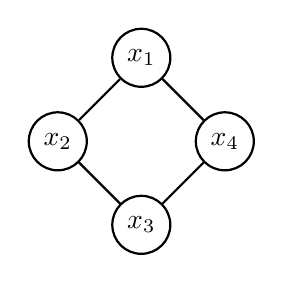
\begin{tikzpicture}[node distance={15mm}, thick, main/.style = {draw, circle}] 
            \node[main] (1) {$x_1$}; 
            \node[main] (2) [below left of=1] {$x_2$};
            \node[main] (3) [below right of=2] {$x_3$}; 
            \node[main] (4) [above right of=3] {$x_4$};
            \draw (1) -- (2);
            \draw (2) -- (3);
            \draw (4) -- (3);
            \draw (1) -- (4);
        \end{tikzpicture}
    \end{minipage}
    \hfill
    \begin{minipage}[c]{.3\linewidth} %inequalities
        \centering
        \begin{gather*}
             \begin{pmatrix}
                1 & 0.9 & ? & -0.9 \\
                0.9 & 1 & 0.9 & ? \\
                ? & 0.9 & 1 & 0.9 \\
                -0.9 & ? & 0.9 & 1
            \end{pmatrix}\\
            S^\G
        \end{gather*}
    \end{minipage}

    \caption{Example from \cite[Section 9.3]{maathuis2018handbook} of a matrix $S$ for which all completely specified submatrices of $S^\G$ are positive definite but which doesn't have a positive definite completion.}
    \label{fig-no-completion}
\end{figure}

However, as shown in the example in Figure \ref{fig-no-completion}, this condition is not sufficient for the existence of a positive definite completion. Still, Grone et al. \cite{GRONE1984109} show that this condition is also sufficient if and only if $\G$ is a chordal graph.
\begin{theorem} \label{thm-chordal-iff}
    For a graph $\G$, the following statements are equivalent.
    \begin{enumerate}[i.]
        \item A partial matrix $M^\G$ has a positive definite completion if and only if all completely specified submatrices of $M^\G$ are positive definite.
        \item $\G$ is chordal.
    \end{enumerate}
\end{theorem}
A consequence of this theorem is that if $\G$ is a chordal graph, then $\t{mlt}(\G) = q(\G)$. This result for chordal graphs can be used to compute an upper bound on the maximum likelihood treshold of a general graph, tighter than the worst-case bound in (\ref{eq-pessimistic-mlt}). 

Let $\G = (\Gamma, E)$ be a graph and $S$ a sample covariance matrix. A graph $\G^+ = (\Gamma, E^+)$ is called a \textit{chordal cover} of $\G$ if $E \subset E^+$ and $\G^+$ is chordal. Then, since $E \subset E^+$, we have that the $\G^+$-partial matrix $S^{\G^+}$ agrees with the $\G$-partial matrix $S^\G$ on the entries corresponding to the edges $E$ of $\G$. Thus, one can view $S^{\G^+}$ as a partial completion of $S^\G$, and any positive definite completion of $S^{\G^+}$ is a valid positive completion of $S^\G$. Hence, by Theorem \ref{thm-chordal-iff}, the following bound holds
\begin{equation*}
    \t{mlt}(\G) \leq q^+(\G) = \min \eset{ q(\G^+) : \G^+ \t{ is a chordal cover of } \G }.
\end{equation*}
Combining (\ref{eq-mlt-upper-bound}) and the above bound, it follows that for any graph $\G$,
\begin{equation} \label{eq-mlt-bounds}
    q(\G) \leq \t{mlt}(\G) \leq q^+(\G).
\end{equation}

\begin{figure}    
    \center
    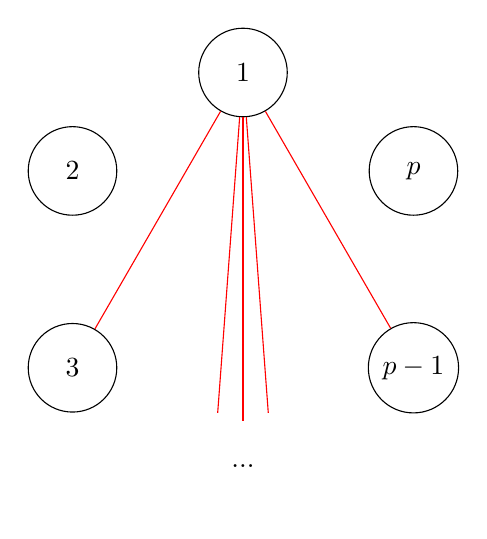
\begin{tikzpicture}[
        point/.style={circle,draw,minimum size=#1},
        point/.default=0pt
    ]
        % \coordinate[label = above:1] (1) at (90:3);
        % \node at (1)[circle,fill,inner sep=2pt]{};

        \node[point=3.2em] (1) at (90:2.5) {1};
        \node[point=3.2em] (2) at (150:2.5) {2};
        \node[point=3.2em] (3) at (210:2.5) {3};
        \node[point=3.2em, draw=none] (dots) at (270:2.5) {...};
        \node[point=3.2em] (pm1) at (330:2.5) {$p-1$};
        \node[point=3.2em] (p) at (30:2.5) {$p$};


        \centerarc[](0,0)(105:135:2.5)
        \centerarc[](0,0)(165:195:2.5)
        \centerarc[](0,0)(225:255:2.5)
        \centerarc[](0,0)(285:314.5:2.5)
        \centerarc[](0,0)(345.5:375:2.5)
        \centerarc[](0,0)(45:75:2.5)

        \draw (1) edge[red] (3);
        \draw (1) edge[red] (dots);
        \draw (1) edge[red] (pm1);
        \draw (1) edge[red] (260:1.85);
        \draw (1) edge[red] (280:1.85);
        
    \end{tikzpicture}
    \caption{The graph $\G = ([p], E)$ formed from the black edges in the above figure is the cycle of length $p$. If $E^+$ is formed by adding the red edges in the figure to $E$, $\G^+ = ([p], E^+)$ forms a chordal cover of $\G$.}
    \label{fig-pcycle}
\end{figure}

\begin{example} \label{ex-pcycle}
    Let $\G = ([p], E)$ be a chordless cycle of length $p \geq 4$, $E = \eset{ \eset{1, 2}, \eset{2, 3}, \ldots, \eset{p, 1}}$. Then, the maximal clique size of $\G$ is $q(\G) = 2$. We can form a chordal cover $\G^+ = ([p], E^+)$ that attains the minimum $q(\G^+) = 3$ by connecting an arbitrary node $a \in [p]$ to all other nodes of $\G$ that are not already neighbours of $a$. That is, we define the set of edges of $\G^+$ by $E^+ = E \cup \eset{ \eset{a, i} : i \in [p] \setminus \eset{a}}$. This chordal covering is depicted in Figure \ref{fig-pcycle}, with $a = 1$. Hence, for a chordless cycle $\G$ of size $p$,
    \begin{equation*}
        2 \leq \t{mlt}(\G) \leq 3.
    \end{equation*}
    The exact conditions under which the maximum likelihood estimator in a chordless cycle exists for $n = 2$ are studied in Buhl \cite[Section 4]{Buhl1993OnTE}.
\end{example}


Now that we have presented some of the conditions under which one can almost surely find a positive definite completion to the $\G$-partial correlation matrix $S^\G$, we turn ourselves to the question of finding an algorithm capable of computing the maximum likelihood estimator $\hat\Sigma$ of $\Sigma$. As discussed earlier, the completely specified principal submatrices of $S^\G$ are the submatrices corresponding to the cliques of $\G$. Hence, finding a positive definite completion of $\S^\G$ is equivalent to finding the matrix $\hat\Sigma$ satisfying for all $C \in \c(C)(\G)$,
\begin{equation} \label{eq-clique-constraint}
    \hat\Sigma_C = S_C.
\end{equation}
This equation naturally suggests an iterative algorithm by successively adjusting parts of the covariance matrix to satisfy (\ref{eq-clique-constraint}) while keeping the running matrix positive definite. This procedure, called \textit{iterative proportional scaling}, was studied by Speed and Kiiveri \cite{speed1986gaussian}, among with other algorithms for solving the maximum equation problem in Gaussian graphical models.

Next, we present a development of the algorithm in a Gaussian graphical model with graph $\G$, given a sample covariance matrix $C$ computed from a sample of size $n > \t{mlt}(\G)$. Let $\Omega \in \S^p_{\succ 0}$ be a positive definite matrix and let $C \in \c{C}(\G)$ be a clique of $\G$. We define the \textit{$C$-marginal adjustment} operator $T_C$ given by
\begin{equation} \label{eq-tc-1}
    T_C \Omega = \Omega + \begin{pmatrix}
        (S_C)^{-1} - (\Sigma_C)^{-1} & 0\\
        0 & 0 
        \end{pmatrix},
\end{equation}
where the variable $\Sigma$ denotes the inverse of $\Omega$, and for simplicity of notation, the top-left block of matrices writen out explicitly corresponds to the current clique $C$. We now show that the operator $T_C$ satisfies the following useful properties.


% \begin{lemma} \label{lem-sym-psd}
%     Let $\Sigma \in \S^p$ be a symmetric block diagonal matrix decomposing as
%     \begin{equation*}
%         \Sigma = \begin{pmatrix}
%             A & B\\
%             B^\top & C
%         \end{pmatrix}.
%     \end{equation*}
%     Then, $\Sigma \in \S^p_{\succ 0}$ if and only if both $E = A - BC^{-1}$ and $C$ are positive definite.
% \end{lemma}

% \begin{proof}
%     See 
% \end{proof}

\begin{proposition}
    Let $\G = ([p], E)$ and $S$ be an empirical covariance matrix constructed from a sample of size $n > \t{mlt}(\G)$ from the Gaussian graphical model associated to $\G$. Then, the operator $T_C$ satisfies the following properties.
    \begin{enumerate}[i.]
        \item $T_C$ is well defined;
        \item $T_C$ adjusts the $C$-marginal of $\Omega$. That is, $(T_C \Omega)^{-1}$ satisfies (\ref{eq-clique-constraint}) for the clique $C$;
        \item If $\Omega \in \S^p_{\succ 0}$, then $T_C \Omega \in \S^p_{\succ 0}$;
        \item If $\Omega \in \S(\G)$, then $T_C \Omega \in \S(\G)$.
    \end{enumerate}    
\end{proposition}
\begin{proof}
    (i) By assumption on the sample size $n$, all matrices and submatrices involved in $T_C$ are positive definite and can be inverted.
    \newline
    (ii) As seen earlier, the inverse of $\Sigma_C$ can be expressed in terms of $\Omega$ by using the Schur complement
    \begin{equation*}
        (\Sigma_C)^{-1} = \Omega_C - \Omega_{C, C^c}(\Omega_{C^c})^{-1}\Omega_{C^c, C},
    \end{equation*}
    where $C^c = [p] \setminus C$ is the complement of $C$ in $[p]$. Replacing this in the definition of $T_C$ gives
    \begin{equation} \label{eq-tc-2}
        T_C \Omega = \begin{pmatrix}
            (S_C)^{-1} + \Omega_{C, C^c}(\Omega_{C^c})^{-1}\Omega_{C^c, C} & \Omega_{C, C^c}\\
            \Omega_{C^c, C} & \Omega_{C^c, C^c}
            \end{pmatrix}.
    \end{equation}
    We can now use the Schur complement to compute the $C$-marginal of $\Omega$,
    \begin{align*}
        \left[(T_C \Omega)^{-1}\right]_C 
        &= \left[ (S_C)^{-1} + \Omega_{C, C^c}(\Omega_{C^c})^{-1}\Omega_{C^c, C} - \Omega_{C, C^c}(\Omega_{C^c})^{-1}\Omega_{C^c, C} \right]^{-1}\\
        &= \left[ (S_C)^{-1}\right]^{-1} = S_C.
    \end{align*}
    (iii) In \cite[Proposition B.1]{lauritzen1996}, Lauritzen gives a sufficient condition for a symmetric diagonal to be positive definite. Applying this proposition, we have that $T_C \Omega$ is positive definite if and only if both $(T_C \Omega)_C$ and $E = (T_C \Omega)_C - (T_C \Omega)_{C, C^c}((T_C \Omega)_{C^c})^{-1}(T_C \Omega)_{C^c,C}$ are positive definite. As seen in (ii), $(T_C \Omega)_C = S_C$ is by assumption positive definite. As for the Schur complement,
    \begin{align*}
        E &= (T_C \Omega)_C - (T_C \Omega)_{C, C^c}((T_C \Omega)_{C^c})^{-1}(T_C \Omega)_{C^c,C}\\
        &= (S_C)^{-1} + \Omega_{C, C^c}(\Omega_{C^c})^{-1}\Omega_{C^c, C} - \Omega_{C, C^c}(\Omega_{C^c})^{-1}\Omega_{C^c,C}\\
        &= (S_C)^{-1},
    \end{align*}
    is by the same assumption positive definite. Hence $T_C \Omega$ is positive definite.
    \newline
    (iv) Let $E$ be the set of edges of $\G$ and $e = \eset{i, j} \notin E$ be a missing edge in $\G$. Since $C$ is a clique of $\G$, we have that $|C \cap \eset{i, j}| \leq 1$ and the entry of the matrix $T_C \Omega$ corresponding to the edge $\eset{i, j}$ is in one of the following submatrices: $(T_C \Omega)_{C, C^c}$, $(T_C \Omega)_{C^c}$ or $(T_C \Omega)_{C^c,C}$. Since these submatrices are left invariant under $T_C$, we have that $(T_C \Omega)_{ij} = \Omega_{ij} = 0$, thus $T_C \Omega \in \S(\G)$.
\end{proof}

Given these properties, we can naturally define an algorithm by cycling through the cliques $C \in \c{C}(\G)$ of $\G$, successively adjusting each $C$-marginal by applying the adjustment operator $T_C$, and repeating until convergence. This algorithm is the iterative proportional scaling algorithm, given in Algorithm \ref{alg:itpropscale}. The question remains of whether this algorithm converges and why. We start by showing that the $C$-marginal adjustment operator computes the solution to a constrained version of (\ref{eq-primal}). A proof of this lemma can be found within the proof of \cite[Theorem 5.4]{lauritzen1996}.

\begin{algorithm}[t!]
    \caption{Iterative proportional scaling}
    \label{alg:itpropscale}
    \begin{algorithmic}[1]
    \Require{Set of cliques $\c{C}(\G)$, sample covariance matrix $S$, tolerance $\varepsilon$.} 
    \Ensure{Maximum likelihood estimator $\hat\Omega$.}
    
        \State {Let $\Omega^0 = 1_p$}
        \State {Let $\Omega^1 = \Omega^0$}
        \For{\texttt{$C \in \c{C}(\G)$ }}
            \State{Set $\Omega^1 := T_C \Omega^1$ }
        \EndFor
        \If{$\norm{\Omega^1 - \Omega^0} < \varepsilon$}
            \State{Return $\hat\Omega := \Omega^1$}
        \Else
            \State{Set $\Omega^0 := \Omega^1$}
            \State{Go to line 2.}
        \EndIf
    \end{algorithmic}
\end{algorithm}

\begin{lemma} \label{lem-tc-sol-opt}
    Let $\Omega^0 \in \S_{\succ 0}(\G)$. The $C$-marginal adjustment operator $T_C$ computes the solution to problem (\ref{eq-primal}) over the section 
    \begin{equation*}
        \Theta_C(\Omega^0) = \eset{ \Omega \in \S_{\succ 0}(\G) : \Omega_{C^c} = \Omega^0_{C^c} \t{ and } \Omega_{C, C^c} = \Omega^0_{C, C^c} }.
    \end{equation*}
    That is, $T_C \Omega^0$ is the solution to
    \begin{align} \label{eq-sub-optim}
        \begin{split}
            &\underset{\Omega \in \S_{\succ 0}(\G)}{\t{maximize}}\ \  \log |\Omega| - \tr[S\Omega]\\
            &\t{subject to}\ \ \Omega_{C^c} = \Omega^0_{C^c} \t{ and } \Omega_{C, C^c} = \Omega^0_{C, C^c}.
        \end{split}
    \end{align}
\end{lemma}
\begin{proof}
    Using the expression of the determinant of a block matrix in terms of Schur complement, we have that
    \begin{equation*}
        \abs{\Omega} 
        = \abs{\Omega_C - \Omega_{C, C^c}(\Omega_{C^c})^{-1}\Omega_{C^c, C}} \abs{\Omega_{C^c}}.
    \end{equation*}
    Furthermore, using the fact that $\Omega \in \Theta(\Omega^0)$, it follows that
    \begin{align*}
        \log \abs{\Omega}
        &= \log \left\{ \abs{\Omega_C - \Omega^0_{C, C^c}(\Omega^0_{C^c})^{-1}\Omega^0_{C^c, C}} \abs{\Omega^0_{C^c}} \right\}\\
        &= \log \abs{\Omega_C - \Omega^0_{C, C^c}(\Omega^0_{C^c})^{-1}\Omega^0_{C^c, C}} + \log \abs{\Omega^0_{C^c}}\\
        &= \log \abs{\Omega'} + \log \abs{\Omega^0_{C^c}},
    \end{align*}
    where $\Omega' = \Omega_C - \Omega^0_{C, C^c}(\Omega^0_{C^c})^{-1}\Omega^0_{C^c, C}$. Since $\Omega^0_{C^c}$ is constant in the optimization problem (\ref{eq-sub-optim}), it can be ignored and we have that $\log \abs{\Omega}$ and $\log \abs{\Omega'}$ are equal up to a constant term. Furthermore, using again the fact that $\Omega \in \Theta_C(\Omega^0)$, we get
    \begin{align*}
        \trB{\Omega S}
        &= \trB{\Omega_C S_C} + \trB{\Omega_{C^c} S_{C^c}} + 2 \trB{\Omega_{C,C^c} S_{C,C^c}} 
        \doteq \trB{\Omega_C S_C} \\
        &= \trB{\Omega'S_C} + \trB{\Omega^0_{C, C^c}(\Omega^0_{C^c})^{-1}\Omega^0_{C^c, C}S_C}
        \doteq  \trB{\Omega'S_C}.
    \end{align*}
    Hence, the optimization problem (\ref{eq-sub-optim}) is equivalent to 
    \begin{equation*}
        \underset{\Omega' \in \S_{\succ 0}^{|C|}}{\t{maximize}}\ \  \log |\Omega'| - \tr[S_C\Omega'].
    \end{equation*}
    Comparing this to the earlier discussions, this problem is equivalent to finding the maximum likelihood estimator of the precision matrix $\Omega'$ of the Gaussian graphical model associated to the graph $\G$ restricted to the nodes in $C$. Since $C$ is a clique, the subgraph is complete and the maximum likelihood estimator is given by $\hat\Omega' = (S_C)^{-1}$. Hence, the solution to (\ref{eq-sub-optim}) is given by $\hat\Omega \in \Theta(\Omega^0)$ where
    \begin{align*}
        \hat\Omega_C
        &= \Omega' + \Omega^0_{C, C^c}(\Omega^0_{C^c})^{-1}\Omega^0_{C^c, C}\\
        &= (S_C)^{-1} + \Omega^0_{C, C^c}(\Omega^0_{C^c})^{-1}\Omega^0_{C^c, C}.
    \end{align*}
    Hence, the solution to (\ref{eq-sub-optim}) is $\hat\Omega = T_C \Omega^0$.
\end{proof}

By Lemma \ref{lem-tc-sol-opt}, Algorithm \ref{alg:itpropscale} corresponds to an \textit{iterative partial maximization} algorithm, or block coordinate descent algorithm. Since $T_C$ is a linear transformation, it is continuous. Further, we showed that $T_C$ maps $\S_{\succ 0}(\G)$ onto itself. With these conditions satisfied, Lauritzen \cite[Proposition A.3]{lauritzen1996} proves that the iterative partial maximization algorithm converges, and hence Algorithm \ref{alg:itpropscale}, to the maximum likelihood estimator $\hat\Omega \in \S_{\succ 0}(\G)$.